\documentclass[dvipsnames,tikz]{standalone}
\usepackage{amsmath}
\usepackage{arevmath}
\usepackage{xcolor}
\usepackage{tikz}
\usetikzlibrary{calc}
\usetikzlibrary{decorations.pathreplacing,calligraphy,3d}
\usepackage{tikz-3dplot} 

\tikzset{main/.style={thick, circle, color=black}}

\newcommand{\arrowIn}{
	\tikz \draw[-stealth] (-1pt,0) -- (1pt,0);
}

\begin{document}
	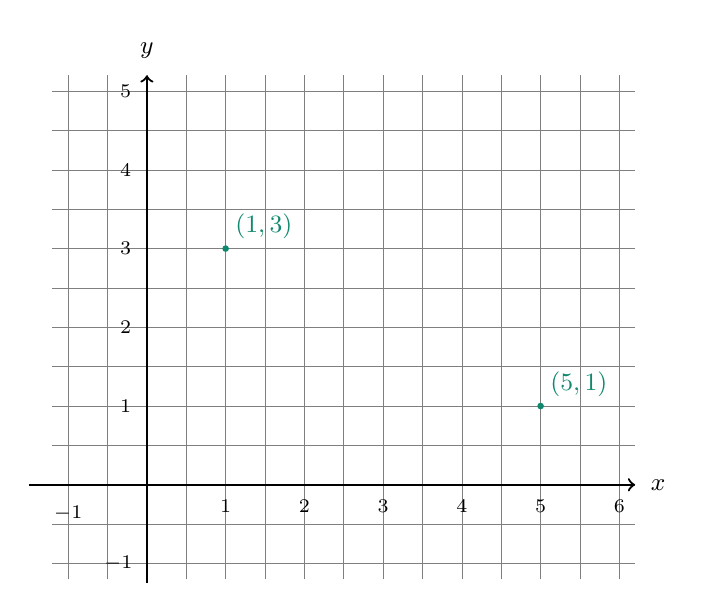
\begin{tikzpicture}[font=\small, tl/.style = {main, inner sep=1pt, font=\scriptsize} ]
		% grid
		\draw[main, very thin, xstep=0.5, ystep=0.5, semitransparent] (-1.2,-1.2) grid (6.2,5.2);
		
		% y tick label
		\foreach \y in {-1,1,2,3,4,5}{
			\node[tl,left=1mm] at (0,\y) {$\y$};
			}
		% x tick label
		\foreach \x in {-1,1,2,3,4,5,6}{
			\node[tl,below=1mm] at (\x,0) {$\x$};
		}
		% axes
		\draw[main, ->,thick] (-1.5,0) -- (6.2,0) node[right] {$x$};
		\draw[main, ->,thick] (0,-1.25) -- (0, 5.2) node[above] {$y$};
		
		% curve
		%\draw[thick, BurntOrange] (1,3) -- (1,1) node[sloped, pos=0.475, scale=1.25, allow upside down]{\arrowIn} -- (5,1) node[sloped, pos=0.475, scale=1.25, allow upside down]{\arrowIn};
		%\draw[thick,PineGreen,domain=-1.2:6.2,variable=\x] plot(\x,3.5-0.5*\x);
		\fill[PineGreen] (1,3) circle (1.2pt) node [above right] {$(1,3)$};
		\fill[PineGreen] (5,1) circle (1.2pt) node [above right] {$(5,1)$};		
	\end{tikzpicture}
	
	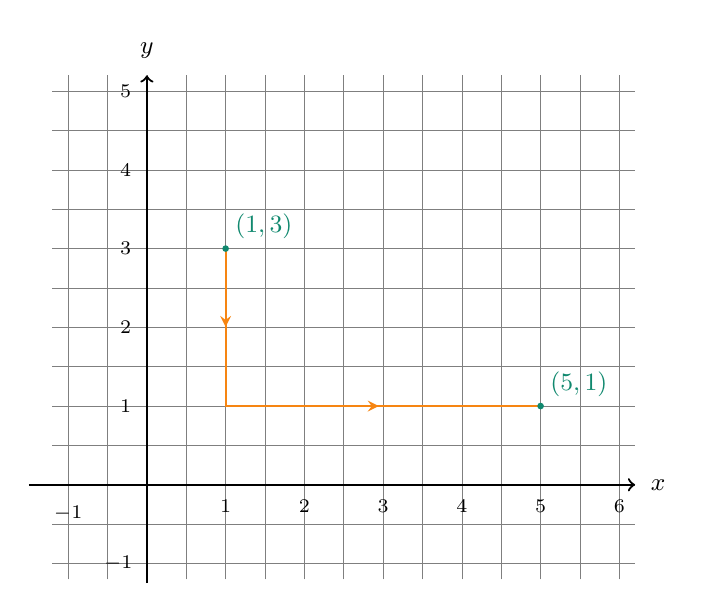
\begin{tikzpicture}[font=\small, tl/.style = {main, inner sep=1pt, font=\scriptsize} ]
		% grid
		\draw[main, very thin, xstep=0.5, ystep=0.5, semitransparent] (-1.2,-1.2) grid (6.2,5.2);
		
		% y tick label
		\foreach \y in {-1,1,2,3,4,5}{
			\node[tl,left=1mm] at (0,\y) {$\y$};
		}
		% x tick label
		\foreach \x in {-1,1,2,3,4,5,6}{
			\node[tl,below=1mm] at (\x,0) {$\x$};
		}
		% axes
		\draw[main, ->,thick] (-1.5,0) -- (6.2,0) node[right] {$x$};
		\draw[main, ->,thick] (0,-1.25) -- (0, 5.2) node[above] {$y$};
		
		% curve
		\draw[thick, BurntOrange] (1,3) -- (1,1) node[sloped, pos=0.475, scale=1.25, allow upside down]{\arrowIn} -- (5,1) node[sloped, pos=0.475, scale=1.25, allow upside down]{\arrowIn};
		%\draw[thick,PineGreen,domain=-1.2:6.2,variable=\x] plot(\x,3.5-0.5*\x);
		\fill[fill,PineGreen] (1,3) circle (1.2pt) node [above right] {$(1,3)$};
		\fill[fill,PineGreen] (5,1) circle (1.2pt) node [above right] {$(5,1)$};		
	\end{tikzpicture}
	
	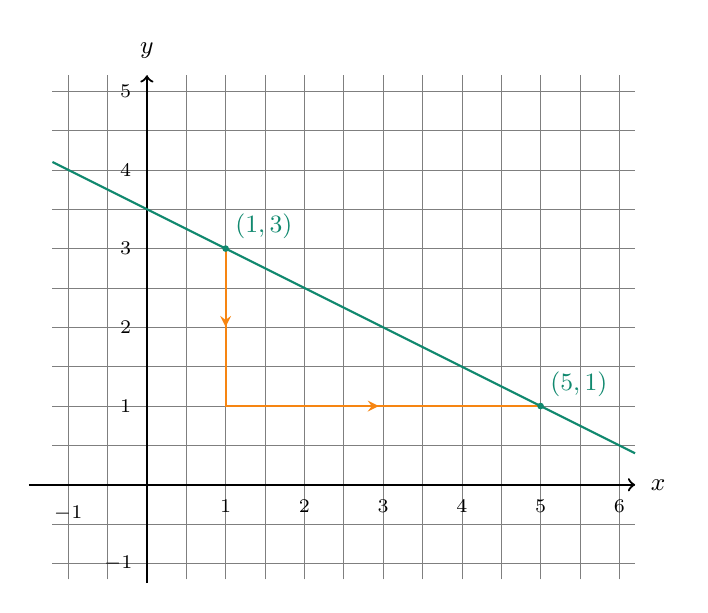
\begin{tikzpicture}[font=\small, tl/.style = {main, inner sep=1pt, font=\scriptsize} ]
		% grid
		\draw[main, very thin, xstep=0.5, ystep=0.5, semitransparent] (-1.2,-1.2) grid (6.2,5.2);
		
		% y tick label
		\foreach \y in {-1,1,2,3,4,5}{
			\node[tl,left=1mm] at (0,\y) {$\y$};
		}
		% x tick label
		\foreach \x in {-1,1,2,3,4,5,6}{
			\node[tl,below=1mm] at (\x,0) {$\x$};
		}
		% axes
		\draw[main, ->,thick] (-1.5,0) -- (6.2,0) node[right] {$x$};
		\draw[main, ->,thick] (0,-1.25) -- (0, 5.2) node[above] {$y$};
		
		% curve
		\draw[thick, BurntOrange] (1,3) -- (1,1) node[sloped, pos=0.475, scale=1.25, allow upside down]{\arrowIn} -- (5,1) node[sloped, pos=0.475, scale=1.25, allow upside down]{\arrowIn};
		\draw[thick,PineGreen,domain=-1.2:6.2,variable=\x] plot(\x,3.5-0.5*\x);
		\fill[fill,PineGreen] (1,3) circle (1.2pt) node [above right] {$(1,3)$};
		\fill[fill,PineGreen] (5,1) circle (1.2pt) node [above right] {$(5,1)$};		
	\end{tikzpicture}
\end{document}